\pdfminorversion=4
\documentclass[aspectratio=169]{beamer}

\mode<presentation>
{
  \usetheme{default}
  \usecolortheme{default}
  \usefonttheme{default}
  \setbeamertemplate{navigation symbols}{}
  \setbeamertemplate{caption}[numbered]
  \setbeamertemplate{footline}[frame number]  % or "page number"
  \setbeamercolor{frametitle}{fg=white}
  \setbeamercolor{footline}{fg=black}
} 

\usepackage[english]{babel}
\usepackage[utf8x]{inputenc}
\usepackage{tikz}
\usepackage{courier}
\usepackage{array}
\usepackage{bold-extra}
\usepackage{minted}
\usepackage[thicklines]{cancel}
\usepackage{fancyvrb}

\xdefinecolor{dianablue}{rgb}{0.18,0.24,0.31}
\xdefinecolor{darkblue}{rgb}{0.1,0.1,0.7}
\xdefinecolor{darkgreen}{rgb}{0,0.5,0}
\xdefinecolor{darkgrey}{rgb}{0.35,0.35,0.35}
\xdefinecolor{darkorange}{rgb}{0.8,0.5,0}
\xdefinecolor{darkred}{rgb}{0.7,0,0}
\definecolor{darkgreen}{rgb}{0,0.6,0}
\definecolor{mauve}{rgb}{0.58,0,0.82}

\title[2021-05-19-vchep-awkwardforth]{{\tt :} AwkwardForth \\ deserialization DSL {\tt +} Awkward-Array {\tt +} {\tt ;}}
\author{Jim Pivarski}
\institute{Princeton University -- IRIS-HEP}
\date{May 19, 2021}

\usetikzlibrary{shapes.callouts}

\begin{document}

\logo{\pgfputat{\pgfxy(0.11, 7.4)}{\pgfbox[right,base]{\tikz{\filldraw[fill=dianablue, draw=none] (0 cm, 0 cm) rectangle (50 cm, 1 cm);}\mbox{\hspace{-8 cm}\includegraphics[height=1 cm]{princeton-logo-long.png}\hspace{0.1 cm}\raisebox{0.1 cm}{\includegraphics[height=0.8 cm]{iris-hep-logo-long.png}}\hspace{0.1 cm}}}}}

\begin{frame}
  \titlepage
\end{frame}

\logo{\pgfputat{\pgfxy(0.11, 7.4)}{\pgfbox[right,base]{\tikz{\filldraw[fill=dianablue, draw=none] (0 cm, 0 cm) rectangle (50 cm, 1 cm);}\mbox{\hspace{-8 cm}\includegraphics[height=1 cm]{princeton-logo.png}\hspace{0.1 cm}\raisebox{0.1 cm}{\includegraphics[height=0.8 cm]{iris-hep-logo.png}}\hspace{0.1 cm}}}}}

% Uncomment these lines for an automatically generated outline.
%\begin{frame}{Outline}
%  \tableofcontents
%\end{frame}

% START START START START START START START START START START START START START

\begin{frame}{Deserializing {\it columnar} data can be very fast}
\vspace{0.25 cm}

\begin{columns}
\column{0.7\linewidth}
\only<1>{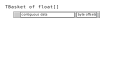
\includegraphics[width=\linewidth]{tbasket-to-awkward-1.pdf}}\only<2>{\includegraphics[width=\linewidth]{tbasket-to-awkward-2.pdf}}\only<3>{\includegraphics[width=\linewidth]{tbasket-to-awkward-3.pdf}}\only<4>{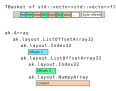
\includegraphics[width=\linewidth]{tbasket-to-awkward-nested.pdf}}

\column{0.3\linewidth}
\begin{onlyenv}<3>''Deserialization'' consists of $\mathcal{O}(1)$ metadata-only operations and $\mathcal{O}(n)$ vectorizable operations.
\end{onlyenv}\begin{onlyenv}<4>Record-oriented data, on the other hand, {\it must} be iterated sequentially, with control-flow decisions throughout.

\vspace{0.5 cm}
For Uproot, this means that reading lists of lists of numbers (in Python) is 460$\times$ slower than reading numbers (NumPy cast).
\end{onlyenv}
\end{columns}
\end{frame}

\begin{frame}{The problem of deserialization}
\Large
\begin{itemize}
\item Data types are not known until you examine the data's schema.
\item The most important part of generating fast code is usually knowing the types.
\end{itemize}

\large
\vspace{0.5 cm}
\begin{columns}[t]
\column{0.5\linewidth}
\mbox{ } \hfill \underline{Common solutions} \hfill \mbox{ }

\vspace{0.25 cm}
JIT-compile the deserialization code.

\vspace{\baselineskip}
\vspace{0.25 cm}
HERE

\column{0.5\linewidth}
\mbox{ } \hfill \underline{Suitable for Uproot?} \hfill \mbox{ }

\vspace{0.25 cm}
Depending on LLVM would undermine portability.

\vspace{0.25 cm}
HERE

\end{columns}
\end{frame}



\end{document}
